\documentclass{report}
\usepackage{graphicx} % Required for inserting images
\usepackage[italian]{babel}
\usepackage{tikz}
\usepackage{hyperref}
\usepackage{amsmath}
\usepackage{xcolor}
\usepackage{float}
\usepackage{soul}
\usepackage{listings} % Per evidenziare il codice

\definecolor{lightgray}{rgb}{0.9,0.9,0.9} % Definizione colore sfondo
\definecolor{darkgreen}{rgb}{0.0, 0.5, 0.0}

\lstset{
    backgroundcolor=\color{lightgray}, % Sfondo grigio
    basicstyle=\ttfamily, % Font monospaziato
    % frame=single, % Bordo attorno al codice
    tabsize=4, % Dimensione tabulazione
    breaklines=true, % Permette di andare a capo automaticamente
    numbers = left,
    numberstyle=\small\color{gray}
}

\title{\huge\textbf{{Integrità delle Query}}}
\date{Parte II}

\begin{document}

\maketitle

\tableofcontents
\newpage

\chapter{Integrità della computazione}

Nel nostro scenario di riferimento potremo avere più \textit{data owner}; queste 
sono entità di cui ci fidiamo.

\noindent Il problema è che questi dati potrebbero essere affidati a dei \textit{cloud provider} esterni, e che possano essere soggetti a delle \textit{computazioni};
questo potrebbe essere un problema sia in termini di confidenzialità che in termini di \textbf{integrità}: 
\textit{"chi mi dice che la tua computazione sia integra?"}.

\section{Esempi}

\subsubsection{Esempio di una query}

Abbiamo l'owner che affida i propri dati ad un provider esterno;
abbiamo poi un client che effettua una query.

\begin{figure}[H]
    \centering
    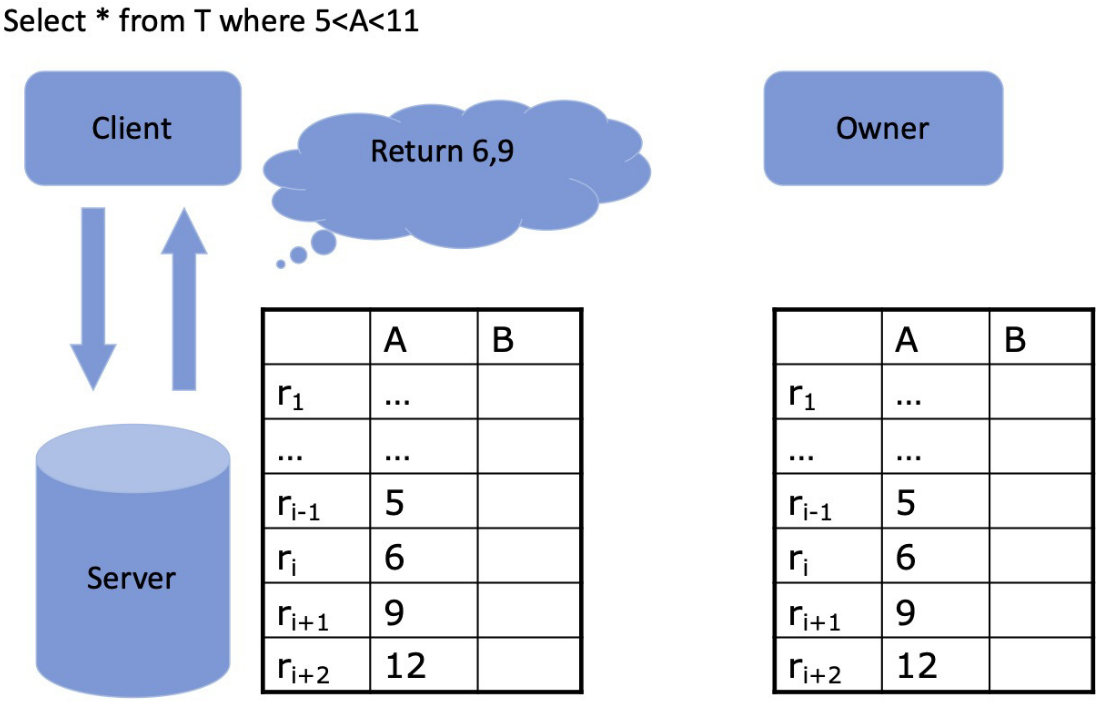
\includegraphics[width=0.7\linewidth]{images/ex1.png}
\end{figure}

\subsubsection{Esempio di query: iniezione}

Viene iniettata un'informazione fasulla; \textit{magari mi 
conviene dirti una cosa piuttosto che un'altra, le tue azioni dipendono 
da quello che ti dico\dots}

\begin{figure}[H]
    \centering
    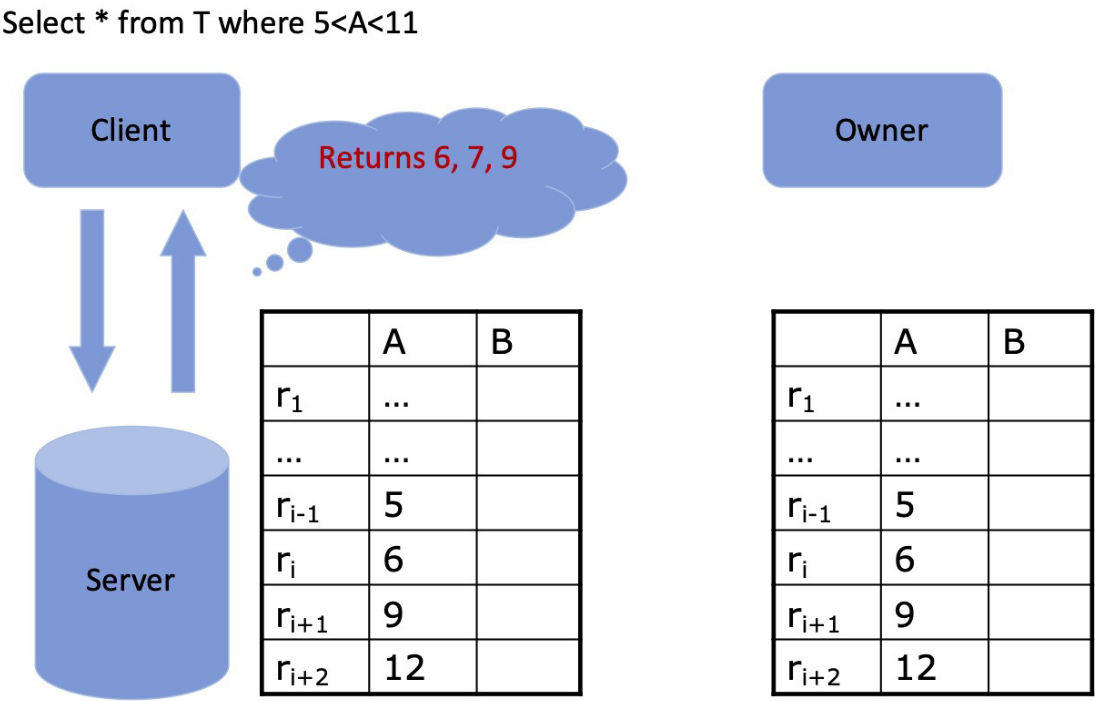
\includegraphics[width=0.9\linewidth]{images/ex2.png}
\end{figure}


\subsubsection{Esempio di query: drop}

\begin{figure}[H]
    \centering
    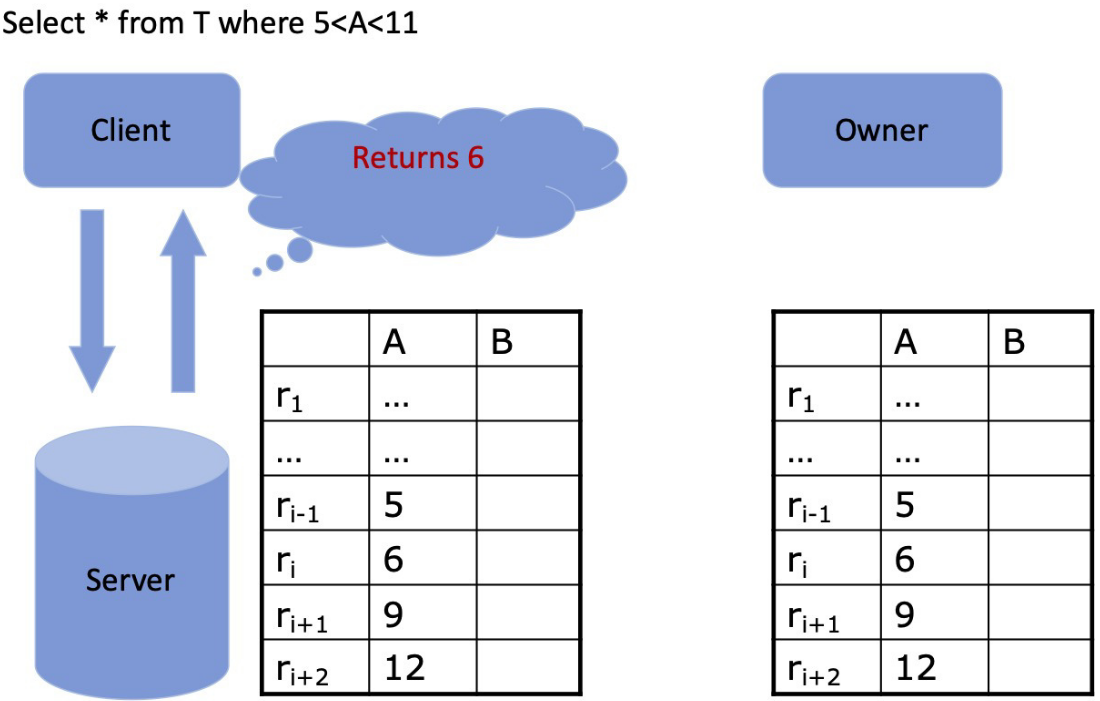
\includegraphics[width=0.9\linewidth]{images/ex3.png}
\end{figure}


\newpage
\subsubsection{Esempio di query: omissione}

I dati potrebbero essere dinamici, dunque potrebbero 
essere richieste delle operazioni di update.

\begin{figure}[H]
    \centering
    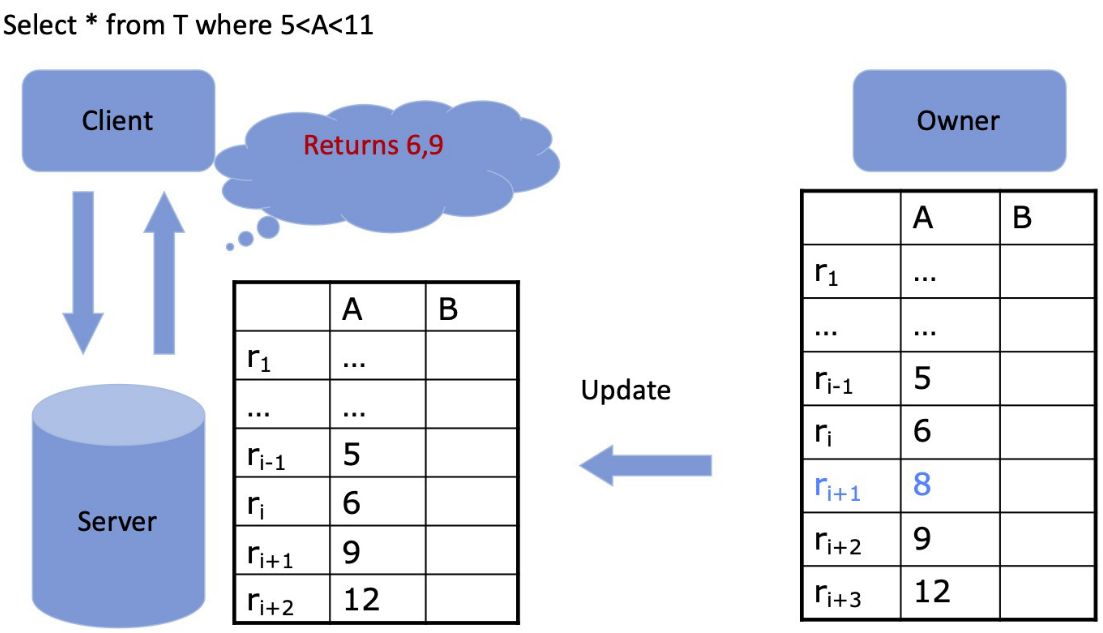
\includegraphics[width=0.9\linewidth]{images/ex4.png}
\end{figure}

\section{Integrità di storage e computazione}

Il data owner e gli utenti necessitano di meccanismi che assicurino l'integrità dei risultati 
delle query. Una query è integra se rispetta:
\begin{itemize}
    \item \textbf{Correttezza:} il risultato viene calcolato sui dati veri dell'owner (primo esempio)
    \item \textbf{Completezza:} il risultato calcolati su tutti i dati (secondo esempio)
    \item \textbf{Freschezza:} il risultato è calcolato sull'ultima versione dei dati che l'owner 
    ha dato (terzo esempio)
\end{itemize}


\noindent Ci sono due diversi tipi di approcci per rispondere al problema di integrità, 
ciascuno con i suoi vantaggi e svantaggi:
\begin{itemize}
    \item \textbf{Deterministico:} \textit{se il risultato di una computazione è integro, sono sicuro 
    al 100\% che sia integro}

    \noindent Queste tecniche vengono implementate in modo che l'owner dà al provider, oltre ai 
    dati da gestire, anche delle strutture ausiliarie che vengono sfruttate per verificare l'integrità della computazione 
    \item \textbf{Probabilistico:} \textit{ti dico sempre se è integro o no, ma non con certezza 
    assoluta ma con una certa probabilità; c'è della probabilità di fare degli errori}

    \noindent Perché si usano questi approcci? Sono tecniche che hanno lo svantaggio di non 
    avere la certezza assoluta ma che hanno altri vantaggi (che vedremo più avanti); il fatto 
    che non avere certezza sia un problema dipende da caso a caso.

    \noindent In queste tecniche il \textit{qualcosa di auisiliario} sono dei "dati finti" (marcatori)
    che "aggiungo" ai dati veri; dalla presenza o meno capisco se la query è integra o no (se prima c'erano e poi 
    non ci sono più, probabilmente c'è un errore)
\end{itemize}

\chapter{Approcci deterministici}

L'idea è che il proprietario \textit{dà fuori} i dati e una struttura 
da lui calcolata. Quando il client vuole fare una computazione, restituisce 
oltre al risultato anche un \textit{qualcosa in più} usando la struttura 
dati; questo prende il nome di 
\textbf{verification object}: è ciò che permette di verificare se il risultato della 
query è integro. 

\begin{figure}[H]
    \centering
    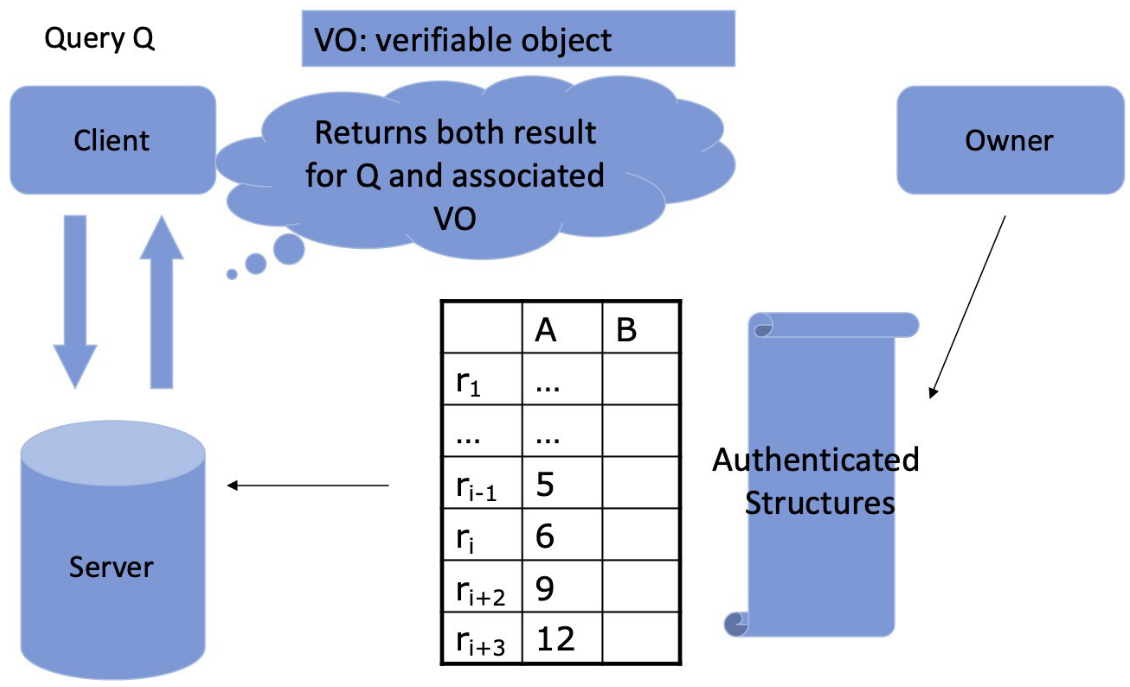
\includegraphics[width=0.8\linewidth]{images/det-idea.png}
\end{figure}

\section{Approccio basato su firma}

Questa tecnica si preoccupa di verificare l'integrità solo per una tipologia
particolare di query, ovvero quelle che coinvolgono un solo attributo 
della relazione; ad esempio $x=5, 4<x<5,\dots$ l'idea è:
\begin{itemize}
    \item ordinare le tuple rispetto al valore dell'attribuo preso in considerazione 
    \item applicare una firma alle tuple, non singolarmente ma in coppie tra loro consecutive 
    
    $(t_1,s_1),(t_2,s_2)\dots(t_n,s_n), con s_i = \epsilon(t_i | t_{i+1})$ 
    \item oltre ai dati, vengono date al provider anche le firme
\end{itemize}

\noindent A questo punto quando un client vuole eseguire una computazione, ad esempio 
$a<x<b$:
\begin{itemize}
    \item vengono restituite le tuple (e le firme associate) $[a-1,b+1] \rightarrow$ voglio anche la tupla 
    immediatamente precedente ed immediatamente successiva 
    \item le \textit{cose aggiunte} al risultato vero e proprio per verificare l'integrità sono: 
    \begin{itemize}
        \item tuple precedente e successiva 
        \item firme associate alle tuple 
    \end{itemize}
\end{itemize} 

\noindent $\Rightarrow$ l'idea è che il client tramite le firme può verificare se il risultato è integro.

\noindent Questo metodo non è molto utilizzato perché:
\begin{itemize}
    \item limitazione sulle query
    \item costosa sia in termini di computazione delle firme, sia nei termini di informazioni 
    aggiuntive che ti devo dare (lineare rispetto al risultato)
\end{itemize}

\begin{figure}[H]
    \centering
    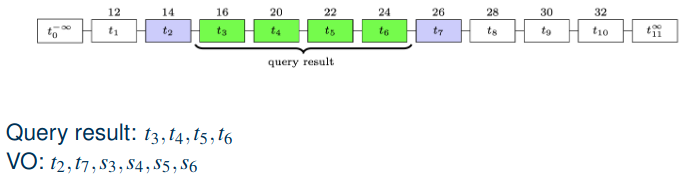
\includegraphics[width=1\linewidth]{images/signature.png}
    \caption{VO sta per verification object}
\end{figure}


\newpage
\section{Merkle hash tree}
Questa tecnica può essere utilizzata per risolvere lo stesso tipo di query viste 
nella sezione precedente, ma in maniera più efficiente. 

\begin{figure}[H]
    \centering
    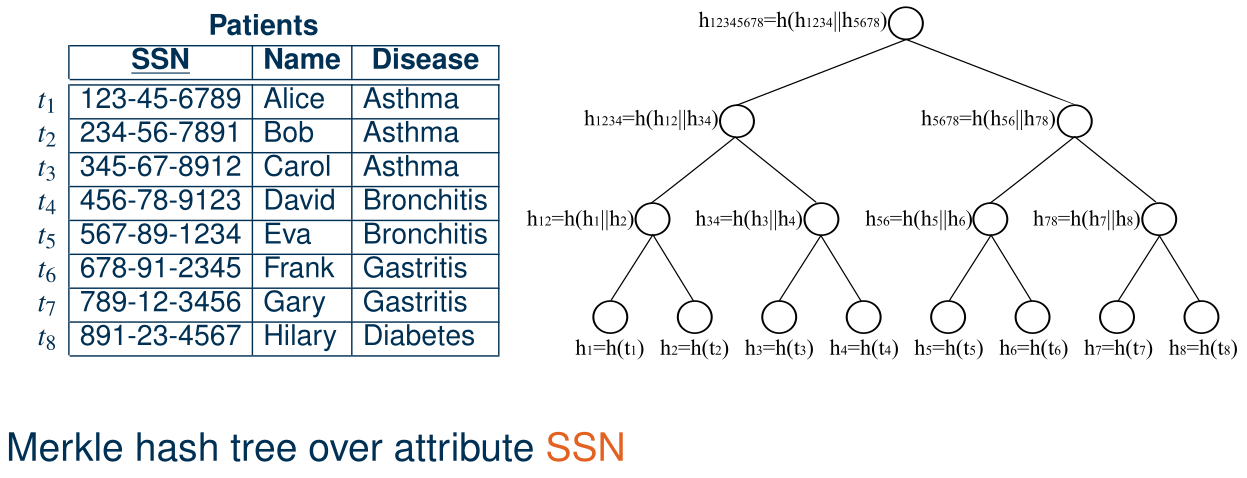
\includegraphics[width=1\linewidth]{images/merkle-hashtree.png}
\end{figure}

L'idea è:
\begin{itemize}
    \item ordinare i valori dell'attributo preso in considerazione
    \item si applica una funzione di hash alle tuple (foglie dell'albero)
    \begin{itemize}
        \item nel livello delle foglie ci sono $2^L$ elementi
        \item i nodi intermedi vengono calcolati applicando la stessa funzione di hash 
        alla concatenazione degli hash dei figli 

        \noindent $\rightarrow$ l'idea è che l'hash di un nodo dipende dall'hash dei figli
        \item se l'albero non è completo, tipicamente si aggiungono delle tuple \textit{null} per renderlo completo 
    \end{itemize}
\end{itemize}

$\Rightarrow$ la quantità di informazioni aggiuntive non è più lineare rispetto al risultato 
ma è \textbf{logaritmica}.

\subsection{Merkle hash tree verification}

\begin{itemize}
    \item L'idea è che il cloud provider fornisce un \textit{\textbf{verification object}} per 
    permettere al client di \textbf{ricostruire l'hash associato alla radice}
    \item Il risultato della query è \textbf{corretto e completo} la radice calcolata 
    corrisponde a quella già conosciuta
    \begin{itemize}
        \item se c'è una tupla mancante o non corretta, la radice calcolata sarà diversa da quella già conosciuta
    \end{itemize}
\end{itemize}

\begin{figure}[H]
    \centering
    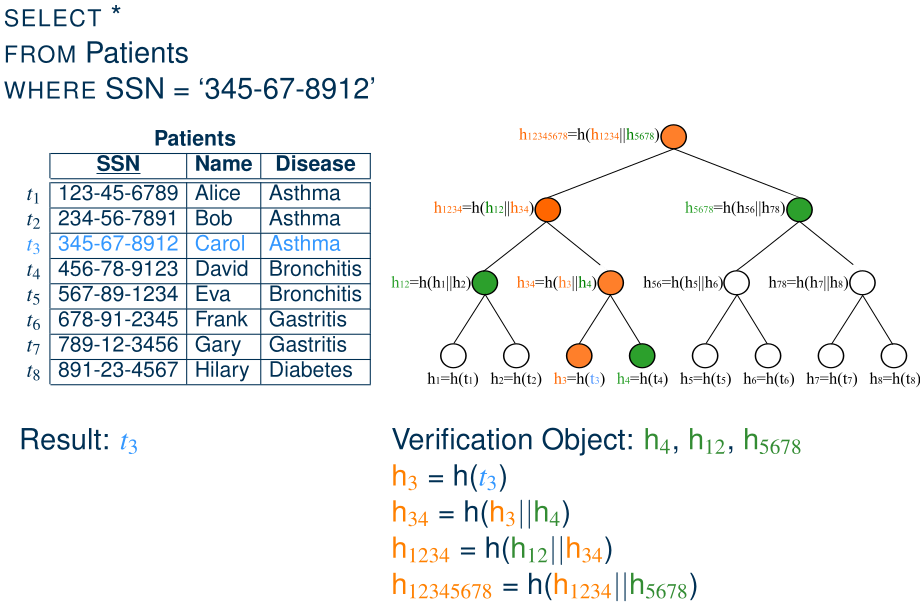
\includegraphics[width=1\linewidth]{images/tree-verification.png}
\end{figure}

\begin{figure}[H]
    \centering
    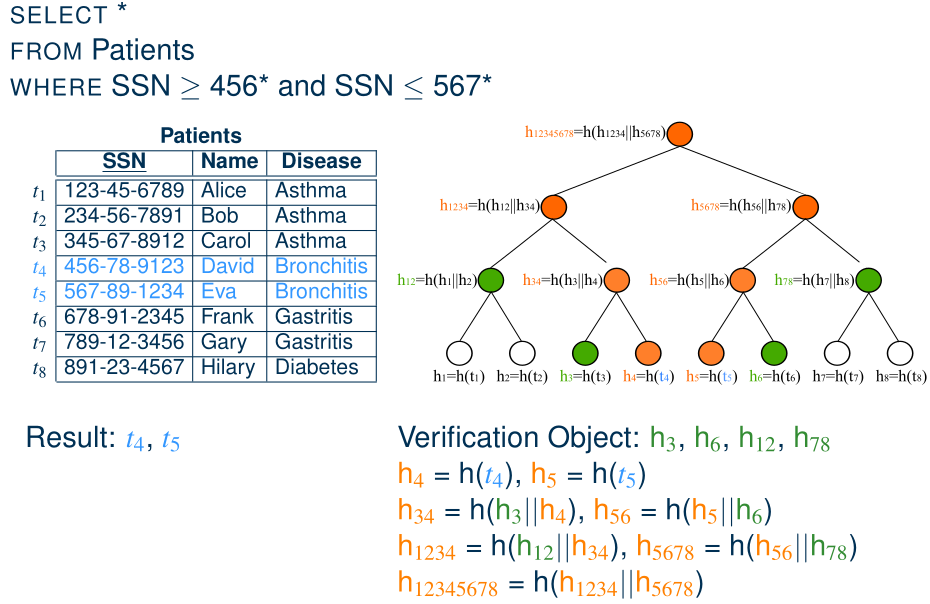
\includegraphics[width=1\linewidth]{images/tree-verification2.png}
\end{figure}

\noindent Con la tecnica delle firme, il costo della verifica è lineare rispetto alla dimensione del risultato; mentre 
con la tecnica dell'albero il costo è sempre pari a $\log n$ (\textit{n numero di foglie})

$\rightarrow$ quando la dimensione del risultato supera $\log n$, sarà più efficiente usare l'albero

\section{Merkle B-tree}
Ciascun nodo contiene più informazioni:
\begin{itemize}
    \item Nodo foglia:
    \begin{itemize}
        \item chiave $k_i$
        \item puntatore all'area di memoria che contiene l'informazione vera e propria 
        \item funzione di hash applicata alla tupla con chiave $k_i$
    \end{itemize}
    \item Nodo interni:
    \begin{itemize}
        \item chiave
        \item puntatori ai nodi figli 
        \item funzione di hash applicata alla concatenazione di tutti gli hash che appaiono nel nodo puntato dal puntatore
    \end{itemize}
\end{itemize}

\begin{figure}[H]
    \centering
    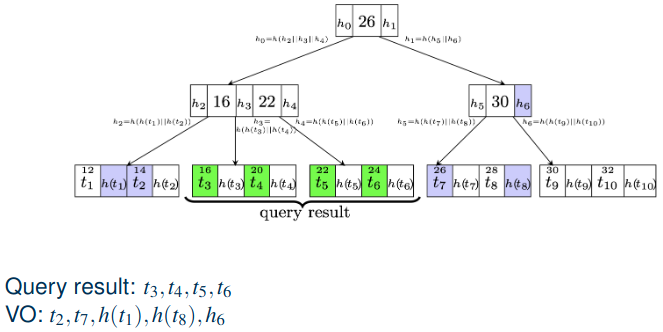
\includegraphics[width=1\linewidth]{images/mb-tree}
\end{figure}

\noindent Per semplicità la tupla nei nodi foglia è memorizzata direttamente all'interno del nodo.

\noindent Concettualmente il meccanismo di funzionamento e verifica è lo stesso dell'albero visto precedentemente; possiamo vedere 
questa versione come una sua generalizzazione in cui ogni nodo può contenere più chiavi.
\begin{itemize}
    \item l'hash associato al nodo radice è un \textit{summary} di tutte le informazioni che contiene l'albero 
\end{itemize}




\section{Skip list}
Ha lo svantaggio che può essere usata solo con query di uguaglianza, ma ha il vantaggio 
di poter essere integrata in modo efficiente in un DBMS.

\noindent Una \textbf{skip list} è una lista



\begin{itemize}
    \item Una \textbf{skip list} per un set di elementi è una serie di liste $S_1, S_2, \dots, S_n$, tale che:
    \begin{itemize}
        \item $S_0$ contiene tutti gli elementi ordinati rispetto a un qualche attributo e le sentinelle $+\infty$ e $-\infty$
        \item $S_i$ contiene un sottoinsieme degli elementi della lista $S_{i-1}$ con una probabilità $p$ (le sentinelle sono sempre inlcuse)
    \end{itemize}
    \item Ha il vantaggio che tutte le operazioni vengono fatte in tempo $O(log(n))$, per cui è molto efficiente
    \begin{itemize}
        \item \texttt{find(x)}
        \item \texttt{delete(x)}
        \item \texttt{insert(x)}
    \end{itemize}
\end{itemize}

\subsection{Search operation}
\begin{itemize}
    \item Si inizia dall'elemento sentinella nella top list ($-\infty$ nella lista più in alto)
    \item Vado avanti finché trovo un valore $\leq$ di quello che sto cercando (\textit{hop forward})
    \item Nel caso in cui ce ne fosse uno maggiore, allora scendo nella lista sotto (\textit{top down}) e proseguo 
    la ricerca con lo stesso procedimento
\end{itemize}

\begin{figure}[H]
    \centering
    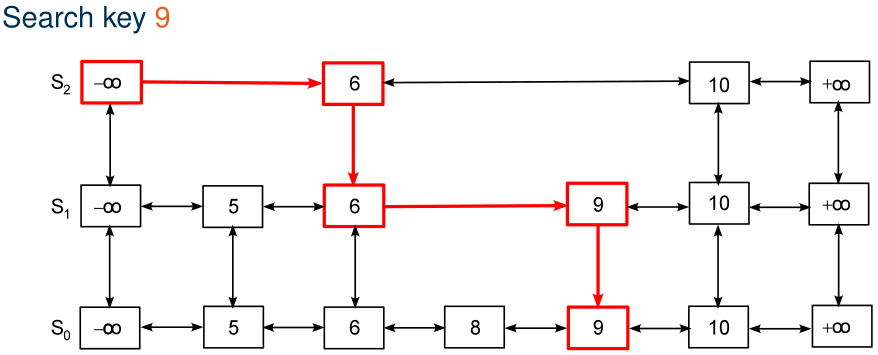
\includegraphics[width=1\linewidth]{images/skip-list.png}
\end{figure}

\subsection{Authenticated skip list}

\noindent Ad ognuno dei nodi si applica una funzione di hash $h$:
\begin{itemize}
    \item resistente a collisioni 
    \item commutativa ($h(x,y)=h(y,x)$)
\end{itemize}

\noindent Ad ogni nodo viene associata una etichetta che, insieme ai \textit{verification object}, permettono di ricostruire il cammino della ricerca 
nel senso opposto, allo scopo di verificare la computazione.

\begin{figure}[H]
    \centering
    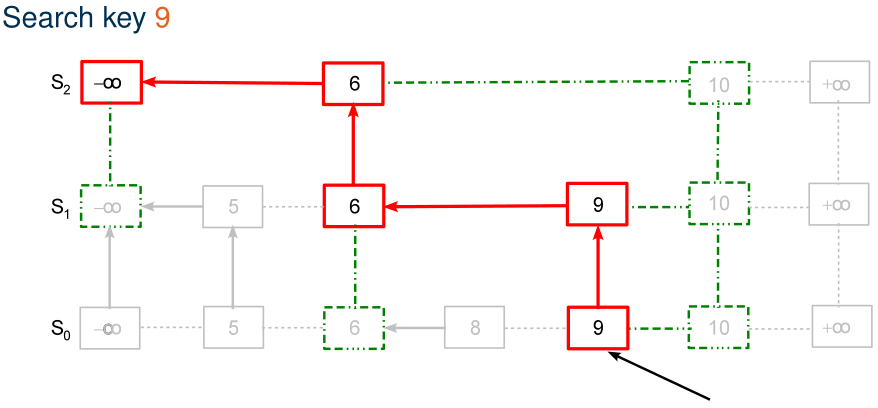
\includegraphics[width=1\linewidth]{images/skip-list-auth.png}
\end{figure}



\chapter{Approcci probabilistici}
Lo svantaggio è che non si ha più la certezza sui risultati, ma hanno il vantaggio di coprire 
più tipologie di query. 


\section{Introduzione}
Possono essere usate due tecniche principali, che possono essere combinate tra loro 
per ottenere una maggiore efficacia.

\subsection{Fake tuples}
L'idea è mettere dentro ai dati originali dei dati fasulli e li mischio; dopo posso controllare 
la loro presenza nel risultato della query (al client restituisco anche le tuple fasulle, lui 
controllerà che ci sono tutte le tuple fasulle che si aspetta).

\noindent Questo meccanismo ha una serie di problematiche che devono essere affrontate:
\begin{itemize}
    \item le tuple \textit{fake} \textbf{non devono essere riconoscibili} da quelle reali 
    \item si utilizzano \textbf{dati criptati} per proteggerli (questo ci aiuta nel punto precedente)
    \item si associa a ciascuna tupla una \textit{informazione aggiuntiva} per verificare l'\textbf{autenticità dei dati}; posso 
    pensare di applicare una funzione di hash alla concatenazione dei valori degli attributi della tupla; questa informazione aggiuntiva 
    la uso anche per distinguere le tuple fasulle da quelle originali
\end{itemize}

\subsubsection{Approccio random}
Quando il client ottiene il risultato di una query, poi deve filtrare le tuple fasulle facendo una 
ulteriore query in locale

$\Rightarrow$ \textcolor{red}{\textbf{il client deve tenersi una copia delle tuple fasulle e computare una query}}

\noindent\dots bisogna pensare ad un altro approccio più efficiente

\subsubsection{Approccio determinstico}
Viene tenuta localmente la funzione usata per generare le tuple fasulle (al posto delle tuple 
fasulle); per semplificare il passo di verifica, l'idea è:
\begin{itemize}
    \item si partizionano i domini
    \item per ogni partizione mi segno quante tuple fasulle gli appartengono 
    \item quando eseguo una query, saprò se una certa partizione del dominio sarà \textit{coperta} parzialmente o completamente dal risultato della query
    \item per verificare farò il conteggio delle tuple fasulle 
\end{itemize}


\begin{figure}[H]
    \centering
    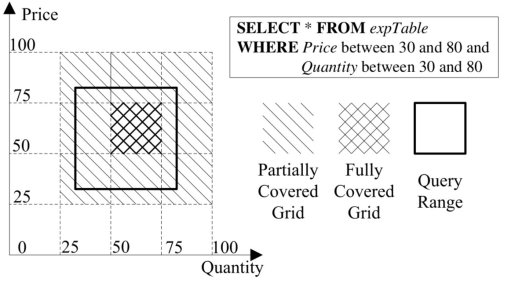
\includegraphics[width=0.8\linewidth]{images/fake-tuples.png}
\end{figure}

\noindent Per calcolare il numero di tuple in una determinata sezione, io conosco 
la funzione usata per generare le tuple; per cui mi basta calcolare i punti 
di intersezione per fare il conteggio (è importante che la funzione sia monotona).

\begin{figure}[H]
    \centering
    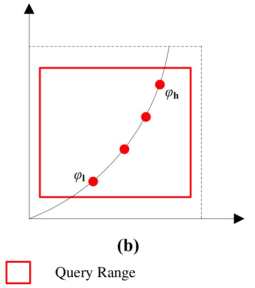
\includegraphics[width=0.4\linewidth]{images/fake-tuples-1.png}
\end{figure}


\subsection{Duplicazione di tuple}
L'idea è quella di non usare tuple fake ma di duplicare alcune tuple reali; la verifica viene 
fatta contando il numero di tuple doppie che mi aspetto di avere. 


\section{Computazione con provider multipli}
Lo scenario di riferimento è quello con multiple sorgenti informative; supponiamo che le 
entità che hanno in mano i dati siano fidate, ma che le computazioni (magari perché sono 
costose) vengano fatte sfruttando le risorse computazionali di qualcun'altro (costa meno 
rispetto a gestirle direttamente).

\noindent Questa entità che gestisce le computazioni non è fidata; anzi, meno costa probabilmente 
meno è fidata \dots devo verificare il risultato che viene restituito.

\noindent In questo contesto vengono combinate le tecniche viste in precedenza.

\begin{figure}[H]
    \centering
    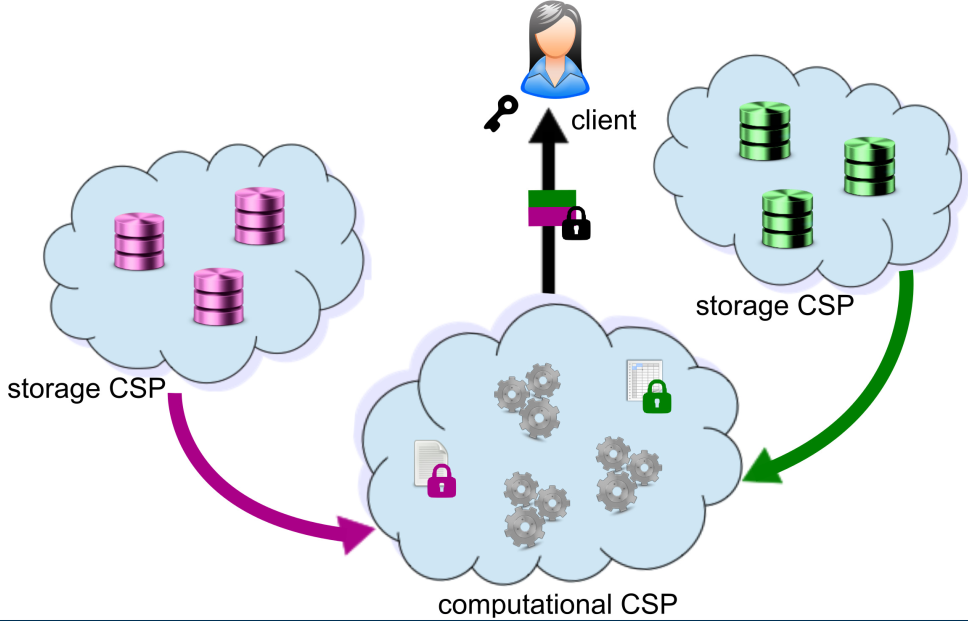
\includegraphics[width=0.8\linewidth]{images/scenario.png}
\end{figure}

\section{Approccio probabilistico per query di join}
Questo tipo di query è quello tipicamente più costoso; le tecniche di protezione 
sono:
\begin{itemize}
    \item \textbf{dati criptati}
    \item \textbf{markers} (tuple fake)
    \item \textbf{twins} (tuple duplicate)
    \item \textbf{salts/buckets} per ottenere occorrenze \textit{flattened}
\end{itemize}


L'idea è:
\begin{itemize}
    \item ho due storage server che sono fidati e che hanno in mano i dati veri e propri
    \item ciascune dei due server mettono dentro \textit{markers} e \textit{twins}
    \item criptano i dati e li danno a \textit{qualcun'alro (computational cloud)}, che non è più 
    grado di distinguere i dati veri da quelli spuri
    \item viene fatta la operazione di join 
    \item chi ha richiesto l'esecuzione della query decripta il risultato, fa tutte le verifiche opportune 
    (markers e twins) e si tiene il risultato
\end{itemize}

\begin{figure}[H]
    \centering
    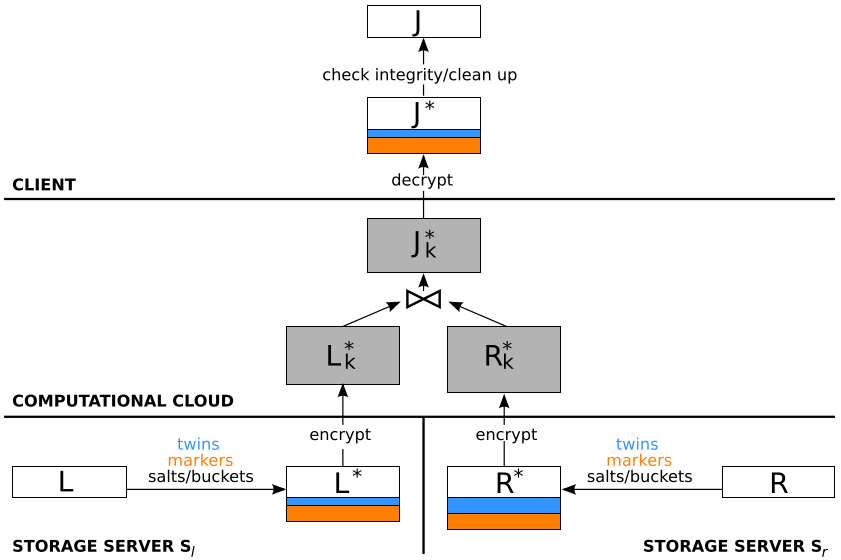
\includegraphics[width=1\linewidth]{images/join.png}
\end{figure}

\subsection{On-the-fly encryption}
La relazione criptata contiene due campi:
mmmmh













\end{document}